\documentclass{article}

\usepackage[a4paper, margin=1.5in]{geometry}
\usepackage[hidelinks]{hyperref}
\usepackage{parskip}
\usepackage{amsmath}
\usepackage{amssymb}
\usepackage{amsthm}
\usepackage{graphicx}
\usepackage{caption}
\usepackage{subcaption}

% Definitions
\theoremstyle{definition}
\newtheorem{definition}{Definition}
\newcommand{\definitionautorefname}{Definition}

% Natural numbers
\newcommand{\N}{\mathbb{N}}

% Partial function
\makeatletter
\newcommand{\pto}{}% just for safety
\DeclareRobustCommand{\pto}{\mathrel{\mathpalette\p@to@gets\to}}
\newcommand{\p@to@gets}[2]{%
  \ooalign{\hidewidth$\m@th#1\mapstochar\mkern5mu$\hidewidth\cr$\m@th#1\to$\cr}%
}
\makeatother

% Source and target operators
\newcommand{\src}{\mathtt{src}}
\newcommand{\trg}{\mathtt{trg}}

% Schema elements
\newcommand{\ptype}{\tau}
\newcommand{\ptypes}{\mathcal{T}}
\newcommand{\rtype}{\tau^\mathsf{r}}
\newcommand{\rtypes}{\mathcal{T}^\mathsf{r}}
\newcommand{\otype}{\tau^\mathsf{o}}
\newcommand{\otypes}{\mathcal{T}^\mathsf{o}}
\newcommand{\gtype}{\tau^\mathsf{g}}
\newcommand{\gtypes}{\mathcal{T}^\mathsf{g}}

% Semantics (double brackets)
\newcommand{\lsem}{\ensuremath{[\![}}
\newcommand{\rsem}{\ensuremath{]\!]}}
\newcommand{\sem}[1]{\ensuremath{\lsem #1 \rsem}}

% Undefined
\newcommand{\undefined}{\mathbf{undef}}

\title{Typing Property Graphs}
\author{Nimo Beeren}


\begin{document}

\section{Introduction}

Graph databases have been steadily growing in popularity in recent years, receiving attention in the form of fundamental research as well as practical usage. One of the spearpoints of the graph database is its flexibility. While the traditionally dominant relational datamodel organizes data into tables and requires a fixed schema, graphs offer a simple yet powerful model consisting of nodes and edges which can be structured freely.

However, this freedom comes at a cost. Without a schema, we miss out on opportunities for query optimization \cite{chakravarthy1990logic, meier2013semantic}, we risk degradation of data integrity, and we lack a formally verifiable source of documentation. By bringing back schemas to the graph world, the flexibility of graph databases can be combined with the robustness of relational databases.

The \emph{property graph model} is the predominant data model among graph database systems today. It provides an intuitive way of modeling entities as nodes, and their relationships as edges. Both nodes and edges are associated with labels, and they hold data in the form of key--value pairs known as \emph{properties}. We can imagine local constraints, such as mandatory properties on nodes or edges, as well as constraints on the structure of the graph, such as mandatory edges between nodes. To the best of our knowledge, there exists no published work that addresses the specification and validation of all these types of constraints using a single schema formalism.

Our overarching goal is to develop an end-to-end framework for property graph schema specification and validation. To this end, we propose a schema formalism capable of expressing local and structural constraints, we provide a prototypical implementation for schema validation in the form of graph queries, and we investigate the practical feasibility of this approach on current graph database systems and realistic datasets.

\section{Property Graphs}

We start by introducing our data model, which is based on the definition of \emph{property graph} established by the Working Group for Database Languages~(WG3) as part of ISO/IEC JTC1/SC32~\cite{deutsch2021gpml}. We use this data model in the rest of this document.

Our notion of property graph represents data as a directed attributed multigraph. Nodes and edges carry data in the form of a set of labels and a set of key--value pairs, called \emph{properties}. We use the umbrella term \emph{objects} to refer to nodes and edges. Being a \emph{multigraph}, a property graph allows the existence of multiple edges between two nodes $u$ and $v$. Furthermore, we allow $u = v$, in which case the edge is called a \emph{self-loop}. For ease of notation, we do not consider undirected edges, although they could be simulated by attaching a special label or property to an edge.

An example of a property graph is given in \autoref{fig:pg}. Nodes are drawn as boxes, and edges are drawn as arrows. Node labels are written in the top compartment, and node properties are written in the bottom compartment. Edge labels are written inside a pill and edge properties are surrounded by `\{' and `\}', which may be omitted when an edge has no properties.

For a formal definition, we assume the existence of the following countably infinite sets: the set of labels $\mathcal{L}$, the set of property names $\mathcal{N}$ and the set of property values $\mathcal{V}$.

\begin{definition}[Basic record]
  \label{def:record-basic}
  A \emph{record} is a finite partial function $r : \mathcal{N} \pto \mathcal{V}$ that maps some property names to property values. The set of all records is denoted as $\mathcal{R}$.
\end{definition}

\begin{definition}[Property graph]
  \label{def:pg}
  A \emph{property graph} is a tuple $$G = (N, E, \rho, \lambda, \pi)$$ where
  \begin{itemize}
    \item $N$ is a finite set of nodes;
    \item $E$ is a finite set of edges such that $N \cap E = \emptyset$;
    \item $\rho : E \to (N \times N)$ is a total function mapping edges to ordered pairs of nodes;
    \item $\lambda : (N \cup E) \to 2^{\mathcal{L}}$ is a total function mapping nodes and edges to a (possibly empty) set of labels;
    \item $\pi : (N \cup E) \to \mathcal{R}$ is a total function mapping nodes and edges to a record.
  \end{itemize}
\end{definition}

Given a node $u$, the set of \emph{outgoing} edges is given by $\{e \in E \mid \exists v \in N : \rho(e) = (u, v)\}$, and the set of \emph{incoming} edges is given by $\{e \in E \mid \exists v \in N : \rho(e) = (v, u)\}$.

The functions $\src$ and $\trg$ map pairs to their first and second element, i.e. $\src((u, v)) = u$ and $\trg((u, v)) = v$. To refer to the source and target \emph{endpoints} of an edge $e$, we may write $\src(\rho(e))$ and $\trg(\rho(e))$ respectively.

\begin{figure}[t]
  \centering
  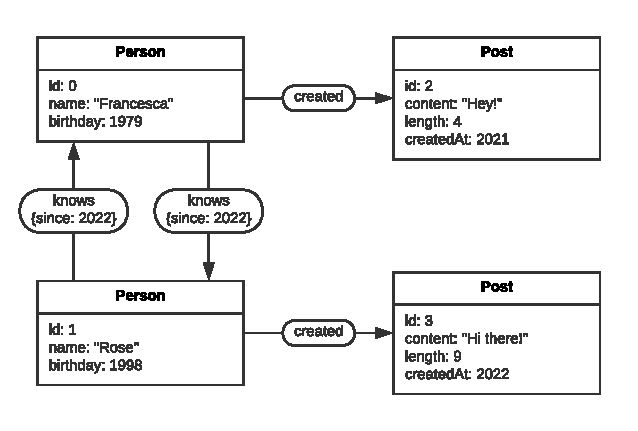
\includegraphics{figures/pg.pdf}
  \caption{A property graph representing a small social network.}
  \label{fig:pg}
\end{figure}

\section{Property Graph Schemas}

A schema should allow modeling of real-world entities and their relationships. A more expressive schema language enables the specification of more complex constraints, but may come at a cost of greater research and engineering effort, as well as worse runtime performance. This needs to be balanced in our choice of schema language.

To explore the schema features that are commonly used in practice, let us look at some existing data modeling techniques. As a baseline, we consider the Entity--Relationship (ER) model as proposed by~\cite{chen1976entity}. This model incorporates entities, relationships, attributes, and values. An \emph{entity} is a ``thing'' that can be uniquely identified, a \emph{relationship} is an association between entities, and an \emph{attribute--value} pair represents information about an entity or relationship. Furthermore, an entity may have a \emph{role} in a relationship, such as ``wife'' or ``husband'' in a marriage relationship. These are the fundamental concepts underlying many data modeling methods in use today.

After the original specification, the ER model has been extended in various ways. For example, a notation which introduced cardinality constraints, optionality, and subtype relations was developed by~\cite{barker1990entity}. With these additions, we can create a more nuanced data model, which more closely matches the real world.

In the next subsection, we first establish a basic definition of property graph schema, which we then extend with additional features such as cardinality constraints (\autoref{sec:cardinality}) and optional properties (\autoref{sec:optional-properties}).

\subsection{Basic definition}

In this subsection, we define a notion of property graph schema which incorporates the basic features of the ER model: entities, relationships, attributes, and values.

\autoref{tab:er-pg} shows how the basic elements of the ER model can be mapped to the property graph model. Note that there are no named roles in the property graph model, but the direction of an edge does allow the distinction between the source and target of an edge. Conversely, the direction of an edge can be represented using roles in the ER model.

\begin{table}[t]
  \centering
  \begin{tabular}{|l|l|}
    \hline
    \textbf{ER} & \textbf{PG} \\
    \hline
    Entity & Node \\
    Relationship & Edge \\
    Attribute & Property name \\
    Value & Value \\
    Role & Edge direction* \\
    \hline
  \end{tabular}
  \caption{Mapping between entity--relationship and property graph concepts. Roles and edge direction can be used for similar purposes, but are not equivalent.}
  \label{tab:er-pg}
\end{table}

An example of a basic property graph schema is given in \autoref{fig:pg-schema-basic}. The similarity between property graphs and schemas allows us to visualize and think about them using the same mental model. Schema nodes and edges are drawn in the same way as for data graphs, but properties are associated with types rather than concrete values.

\begin{figure}[t]
  \centering
  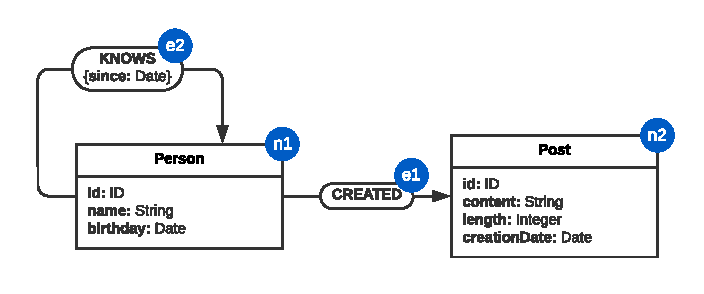
\includegraphics{figures/pg-schema-basic.pdf}
  \caption{A basic property graph schema.}
  \label{fig:pg-schema-basic}
\end{figure}

To formally define property graph schemas and schema conformance, we first assume the existence of a set of property types $\mathcal{T}$. Next, we introduce a number of supporting concepts.

\begin{definition}[Basic property conformance]
  \label{def:property-conformance-basic}
  For each property type $\ptype \in \ptypes$ there is a set $\sem{\ptype} \subseteq \mathcal{V}$ that contains all property values that \emph{conform} to the type $\ptype$.
\end{definition}

\begin{definition}[Basic record type]
  \label{def:record-type-basic}
  A \emph{record type} is a finite partial function $\rtype : \mathcal{N} \pto \ptypes$ that maps some property names to a property type.
  % We denote such record types as $\langle a_1 : \ptype_1, \ldots, a_n : \ptype_n \rangle$.
\end{definition}

\begin{definition}[Basic record conformance]
  \label{def:record-conformance-basic}
  We say that a record $r$ \emph{conforms} to a record type $\rtype$, denoted $r \in \sem{\rtype}$, if for each property name $k \in \mathcal{N}$ it holds that (1) $r(k)$ is defined iff $\rtype(k)$ is defined and (2) $r(k) \in \sem{\rtype(k)}$ if $r(k)$ and $\rtype(k)$ are defined.
\end{definition}

\begin{definition}[Object type]
  \label{def:object-type}
  An \emph{object type} is a pair $\otype = (L, \rtype)$ where $L \subseteq \mathcal{L}$ is a finite set of labels and and $\rtype$ a record type. 
  % We denote such object types also simply as $L\rtype$ or $\{ l_1 \ldots l_k \} \langle a_1 : \rtype_1, \ldots, a_n : \rtype_n \rangle$.
  The set of all object types is denoted as $\otypes$.
\end{definition}

\begin{definition}[Object conformance]
  \label{def:object-conformance}
  Let $G = (N, E, \rho, \lambda, \pi)$ be a property graph and $\otype = (L, \rtype)$ an object type. The set of objects that \emph{conform} to $\otype$ is defined as $\sem{\otype} = \{o \in N \cup E \mid \lambda(o) = L \wedge \pi(o) \in \sem{\rtype}\}$.
\end{definition}

\begin{definition}[Basic property graph schema]
  \label{def:pg-schema-basic}
  A \emph{property graph schema} is a tuple $$\gtype = (N, E, \rho, \omega)$$ where 
  \begin{itemize}
    \item $N$ is a finite set of schema nodes;
    \item $E$ is a finite set of schema edges such that $N \cap E = \emptyset$;
    \item $\rho : E \to (N \times N)$ is a total function mapping schema edges to ordered pairs of schema nodes;
    \item $\omega : (N \cup E) \to \otypes$ is a total function mapping schema objects to object types.
  \end{itemize}
\end{definition}

We may informally say that an object $o$ conforms to a schema object $o'$, by which we mean that $o \in \sem{\omega(o')}$.

Note that a property graph schema can be simulated by a property graph if we allow properties to take property types as values, i.e. $\ptypes \subseteq \mathcal{V}$. Then we let $\lambda$ and $\pi$ take the role of $\omega$, in the sense that $\lambda(o) = L$ and $\pi(o) = \rtype$ if $\omega(o) = (L, \rtype)$ for all objects $o$ in the property graph.

Next, we define the rules that must hold for a property graph to conform to a schema.

\begin{definition}[Basic schema conformance]
  \label{def:schema-conformance-basic}
  Given a property graph $$G = (N, E, \rho, \lambda, \pi)$$ and a property graph schema $$\gtype = (N', E', \rho', \omega)$$ we say that $G$ \emph{conforms} to $\gtype$ if and only if all of the following rules hold.

  \begin{enumerate}
    \item\label{rule:conformance-basic-node}
    Every node $n$ conforms to some schema node $n'$:
    \begin{align*}
      &\forall n \in N \; \exists n' \in N' :\\
      &\quad n \in \sem{\omega(n')}
    \end{align*}
    
    \item\label{rule:conformance-basic-edge}
    Every edge $e$ conforms to some schema edge $e'$, and the endpoints of $e$ conform to the respective endpoints of $e'$:
    \begin{align*}
      &\forall e \in E \; \exists e' \in E' :\\
      &\quad e \in \sem{\omega(e')} \wedge \src(\rho(e)) \in \sem{\omega(\src(\rho'(e')))}\\
      &\quad\quad\wedge \trg(\rho(e)) \in \sem{\omega(\trg(\rho'(e')))}
    \end{align*}
    
    \item\label{rule:conformance-basic-out}
    If a node $n$ conforms to the source of a schema edge $e'$, it must have all the outgoing edges of the right type:
    \begin{align*}
      &\forall n \in N \; \forall e' \in E':\\
      &\quad \big[n \in \sem{\omega(\src(\rho(e')))} \implies \exists e \in E \cap \sem{\omega(e')} :\\
      &\quad\quad \src(\rho(e)) = n \wedge \trg(\rho(e)) \in \sem{\omega(\trg(\rho(e')))}\big]
    \end{align*}

    \item\label{rule:conformance-basic-in}
    If a node $n$ conforms to the target of a schema edge $e'$, it must have all the incoming edges of the right type:
    \begin{align*}
      &\forall n \in N \; \forall e' \in E'  :\\
      &\quad \big[n \in \sem{\omega(\trg(\rho(e')))} \implies \exists e \in E \cap \sem{\omega(e')} :\\
      &\quad\quad \src(\rho(e)) \in \sem{\omega(\src(\rho(e')))} \wedge \trg(\rho(e)) = n\big]
    \end{align*}
  \end{enumerate}
\end{definition}

\autoref{fig:conformance-basic} contains some examples of property graphs which are validated against the schema of \autoref{fig:pg-schema-basic}.

Under these definitions, a schema edge requires that \emph{at least one} conforming edge exists in the property graph. That is, if a schema node has an incident edge (i.e. an incoming or outgoing edge that the schema node participates in), then any node that conforms to the schema node must also have at least one incident edge (in the same direction) that conforms to the schema edge. In the following, we relax this requirement and introduce a more general notion of cardinality constraints.

\begin{figure}[t]
  \centering
  \begin{subfigure}[t]{0.45\textwidth}
    \centering
    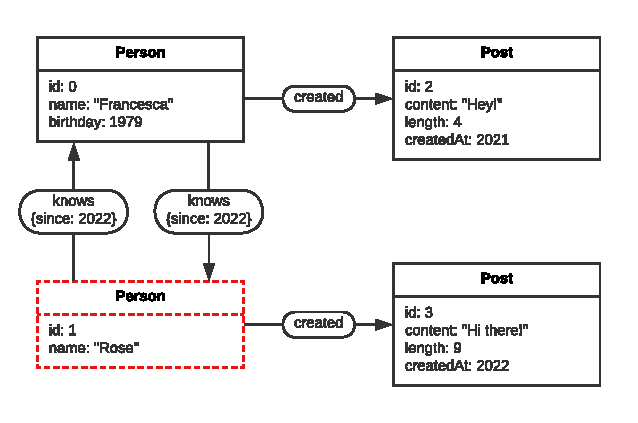
\includegraphics[width=\textwidth]{figures/conformance-basic-node.pdf}
    \caption{A \texttt{Person} is missing a \texttt{birthday}, which violates rule \ref{rule:conformance-basic-node}.}
    \label{fig:conformance-basic-node}
  \end{subfigure}
  \hfill
  \begin{subfigure}[t]{0.45\textwidth}
    \centering
    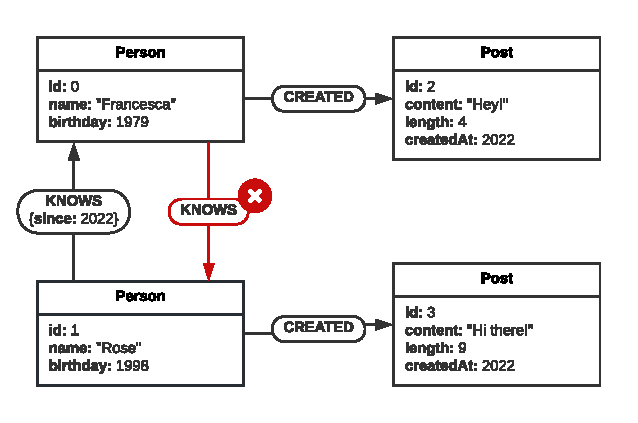
\includegraphics[width=\textwidth]{figures/conformance-basic-edge.pdf}
    \caption{A \texttt{knows} edge is missing a \texttt{since} property, which violates rule \ref{rule:conformance-basic-edge}.}
    \label{fig:conformance-basic-edge}
  \end{subfigure}

  \vskip\baselineskip

  \begin{subfigure}[t]{0.45\textwidth}
    \centering
    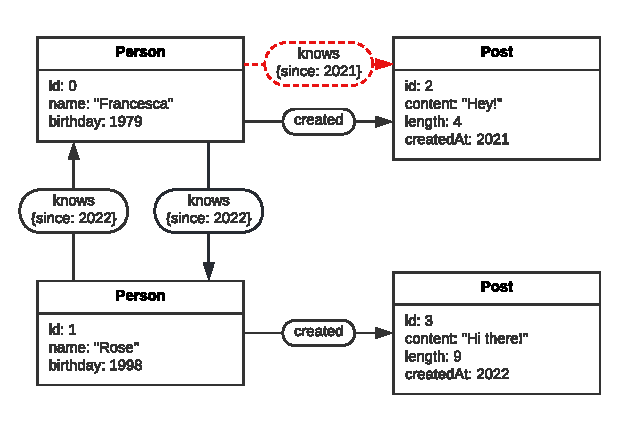
\includegraphics[width=\textwidth]{figures/conformance-basic-edge-target.pdf}
    \caption{The target of a \texttt{knows} edge is not a \texttt{Person}, which violates rule \ref{rule:conformance-basic-edge}.}
    \label{fig:conformance-basic-edge-target}
  \end{subfigure}
  \hfill
  \begin{subfigure}[t]{0.45\textwidth}
    \centering
    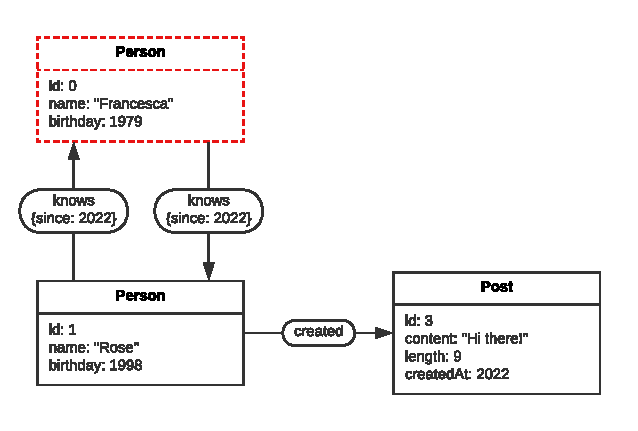
\includegraphics[width=\textwidth]{figures/conformance-basic-out.pdf}
    \caption{A \texttt{Person} is missing an outgoing \texttt{created} edge, which violates rule \ref{rule:conformance-basic-out}.}
    \label{fig:conformance-basic-out}
  \end{subfigure}

  \vskip\baselineskip
  
  \begin{subfigure}[t]{0.45\textwidth}
    \centering
    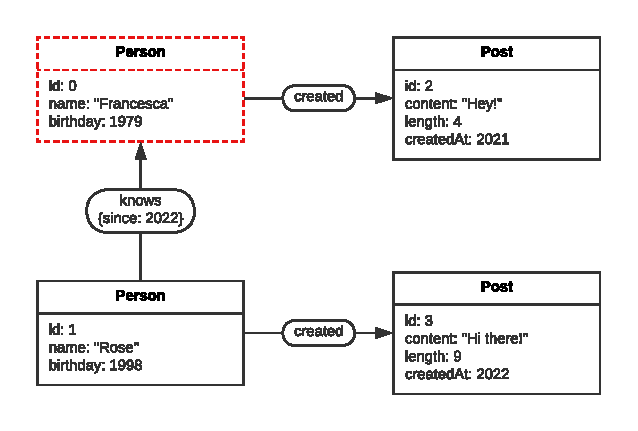
\includegraphics[width=\textwidth]{figures/conformance-basic-out-2.pdf}
    \caption{A \texttt{Person} is missing an outgoing \texttt{knows} edge, which violates rule \ref{rule:conformance-basic-out}.}
    \label{fig:conformance-basic-out-2}
  \end{subfigure}
  \hfill
  \begin{subfigure}[t]{0.45\textwidth}
    \centering
    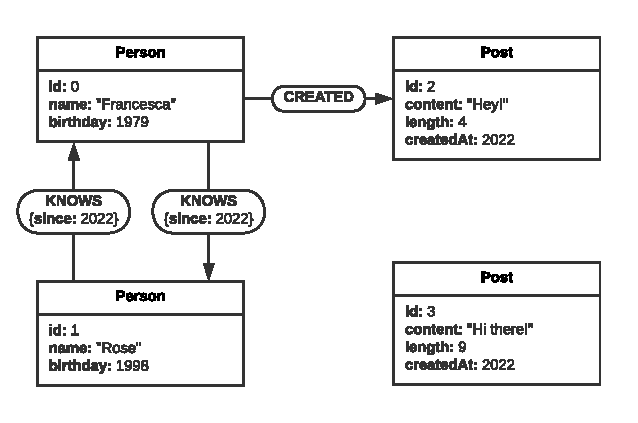
\includegraphics[width=\textwidth]{figures/conformance-basic-in.pdf}
    \caption{A \texttt{Post} is missing an incoming \texttt{created} edge, which violates rule \ref{rule:conformance-basic-in}.}
    \label{fig:conformance-basic-in}
  \end{subfigure}

  \caption{Examples of property graphs that do not conform to the schema of \autoref{fig:pg-schema-basic}. Violating nodes and edges have a red dotted outline.}
  \label{fig:conformance-basic}
\end{figure}

\subsection{Cardinality constraints}
\label{sec:cardinality}

We first introduce a generalization of the existential quantifier which enables counting the number of distinct variables that satisfy a predicate.

\begin{definition}[Counting quantifier]
  The \emph{counting quantifier} is defined as follows. Given two numbers $n, m \in \N$, a predicate $P$, and a set $X$, define
  \begin{itemize}
    \item $\exists^{\geq n} x \in X : P(x) \equiv \exists x_1, \ldots, x_n \in X : P(x_1) \wedge \ldots \wedge P(x_n) \wedge \forall 1 \leq i < j \leq n : x_i \neq x_j$;
    % FIXME: this might be ambiguous, add brackets?
    \item $\exists^{\leq n} x \in X : P(x) \equiv \exists x_1, \ldots, x_n, x_{n+1}, \ldots, x_k \in X : P(x_1) \wedge \ldots \wedge P(x_k) \implies \forall n < i < j \leq k : x_i = x_j$;
    \item $\exists^{[n, m]} x \in X : P(x) \equiv \exists^{\geq n} x \in X : P(x) \wedge \exists^{\leq m} x' \in X : P(x')$;
    \item $\exists^{[n, *]} x \in X : P(x) \equiv \exists^{\geq n} x \in X : P(x)$.
  \end{itemize}
\end{definition}

Next, we introduce the notion of a \emph{cardinality constraint}.

\begin{definition}[Cardinality constraint]
  \label{def:cardinality-constraint}
  A \emph{cardinality constraint} is an ordered pair of intervals $([n_1, m_1], \, [n_2, m_2])$ where $n_1, n_2 \in \N$ and $m_1, m_2 \in \N^*$ with $\N = \{0, 1, 2, \ldots\}$ and $\N^* = \N \cup \{*\}$. The set of all cardinality constraints is denoted as $\mathcal{C}$.
\end{definition}

The two intervals of a cardinality constraint apply to the source and target of an edge, respectively. We also use the functions $\src$ and $\trg$ to refer to the first and second interval of a cardinality constraint, i.e. $\src([n_1, m_1], \, [n_2, m_2]) = [n_1, m_1]$ and $\trg([n_1, m_1], \, [n_2, m_2]) = [n_2, m_2]$.

Next, we revise the definitions of property graph schema and schema conformance, making use of our newly defined cardinality constraints. The following definitions supersede \autoref{def:pg-schema-basic} and~\ref{def:schema-conformance-basic}.

\begin{definition}[Property graph schema]
  \label{def:pg-schema}
  A \emph{property graph schema} is a tuple $$\gtype = (N, E, \rho, \omega, \eta)$$ where
  \begin{itemize}
    \item $N$ is a finite set of schema nodes;
    \item $E$ is a finite set of schema edges such that $N \cap E = \emptyset$;
    \item $\rho : E \to (N \times N)$ is a total function mapping schema edges to ordered pairs of schema nodes;
    \item $\omega : (N \cup E) \to \otypes$ is a total function mapping schema objects to object types;
    \item $\eta : E \to \mathcal{C}$ is a total function mapping schema edges to cardinality constraints.
  \end{itemize}
\end{definition}

An example of a property graph schema with cardinality constraints is given in \autoref{fig:pg-schema}. Intervals such as $[n, m]$ are written as $n..m$, and $[n, n]$ is written simply as $n$, following notation established in UML~\cite{uml}. Furthermore, we use the ``look-here'' notation (as opposed to ``look-across''), meaning that the interval indicates the minimum and maximum number of edges that the node on that side of the edge must participate in. Contrary to some data modeling diagram conventions, the arrow head is unrelated to cardinality, instead it specifies the direction of an edge. Note  that every property graph that conforms to \autoref{fig:pg-schema-basic} also conforms to \autoref{fig:pg-schema}, but not the other way around.

\begin{figure}[t]
  \centering
  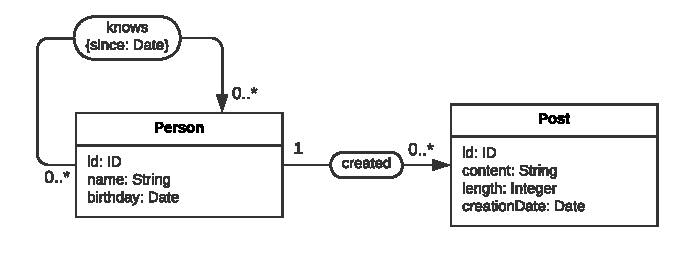
\includegraphics{figures/pg-schema.pdf}
  \caption{A property graph schema with cardinality constraints.}
  \label{fig:pg-schema}
\end{figure}

\begin{definition}[Schema conformance]
  \label{def:schema-conformance}
  Given a property graph $$G = (N, E, \rho, \lambda, \pi)$$ and a property graph schema $$\gtype = (N', E', \rho', \omega, \eta)$$ we say that $G$ \emph{conforms} to $\gtype$ if and only if all of the following rules hold.

  \begin{enumerate}
    \item\label{rule:conformance-node}
    Every node $n$ conforms to some schema node $n'$:
    \begin{align*}
      &\forall n \in N \; \exists n' \in N' :\\
      &\quad n \in \sem{\omega(n')}
    \end{align*}
    
    \item\label{rule:conformance-edge}
    Every edge $e$ conforms to some schema edge $e'$, and the endpoints of $e$ conform to the respective endpoints of $e'$:
    \begin{align*}
      &\forall e \in E \; \exists e' \in E' :\\
      &\quad e \in \sem{\omega(e')} \wedge \src(\rho(e)) \in \sem{\omega(\src(\rho'(e')))}\\
      &\quad\quad\wedge \trg(\rho(e)) \in \sem{\omega(\trg(\rho'(e')))}
    \end{align*}
    
    \item\label{rule:conformance-out}
    If a node $n$ conforms to the source of a schema edge $e'$, it must have the right number of outgoing edges of the right type:
    \begin{align*}
      &\forall n \in N \; \forall e' \in E':\\
      &\quad \big[n \in \sem{\omega(\src(\rho(e')))} \implies \exists^{\src(\eta(e'))} e \in E \cap \sem{\omega(e')} :\\
      &\quad\quad \src(\rho(e)) = n \wedge \trg(\rho(e)) \in \sem{\omega(\trg(\rho(e')))}\big]
    \end{align*}

    \item\label{rule:conformance-in}
    If a node $n$ conforms to the target of a schema edge $e'$, it must have the right number of incoming edges of the right type:
    \begin{align*}
      &\forall n \in N \; \forall e' \in E'  :\\
      &\quad \big[n \in \sem{\omega(\trg(\rho(e')))} \implies \exists^{\trg(\eta(e'))} e \in E \cap \sem{\omega(e')} :\\
      &\quad\quad \src(\rho(e)) \in \sem{\omega(\src(\rho(e')))} \wedge \trg(\rho(e)) = n\big]
    \end{align*}
  \end{enumerate}
\end{definition}

Compared to \autoref{def:schema-conformance-basic}, rules~\ref{rule:conformance-node} and~\ref{rule:conformance-edge} are unchanged, but the counting quantifiers in~\ref{rule:conformance-out} and~\ref{rule:conformance-in} now ensure that nodes do not have too few or too many edges of a particular type.

\autoref{fig:conformance} contains some examples of property graphs which are validated against the schema of \autoref{fig:pg-schema}, taking into account the new rules for cardinality constraints.

\begin{figure}[t]
  \centering
  \begin{subfigure}[t]{0.45\textwidth}
    \centering
    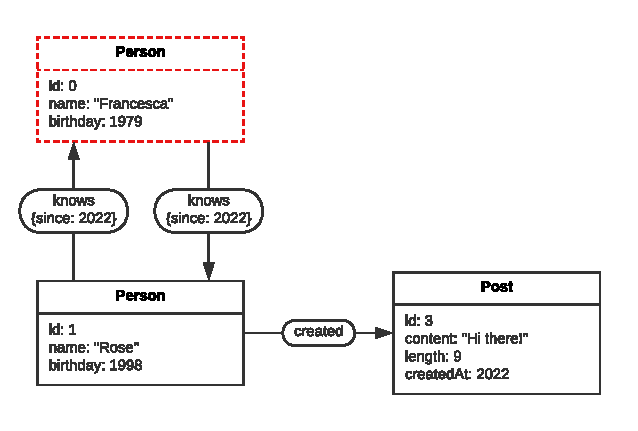
\includegraphics[width=\textwidth]{figures/conformance-out.pdf}
    \caption{Conforms to the schema. A \texttt{Person} is allowed to have created 0 \texttt{Post}s.}
    \label{fig:conformance-node}
  \end{subfigure}
  \hfill
  \begin{subfigure}[t]{0.45\textwidth}
    \centering
    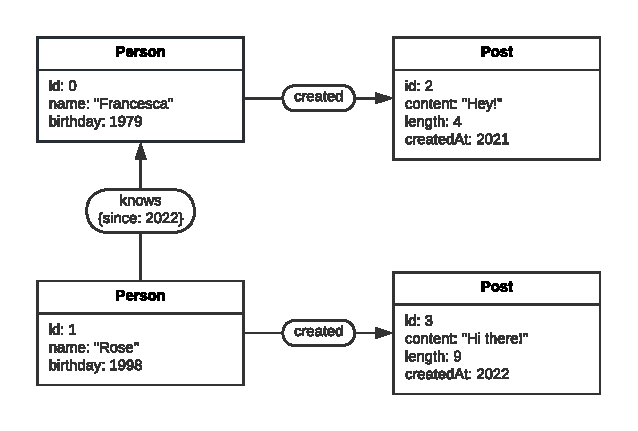
\includegraphics[width=\textwidth]{figures/conformance-out-2.pdf}
    \caption{Conforms to the schema. A \texttt{Person} is allowed to have no outgoing \texttt{knows} edges.}
    \label{fig:conformance-edge}
  \end{subfigure}

  \vskip\baselineskip

  \begin{subfigure}[t]{0.45\textwidth}
    \centering
    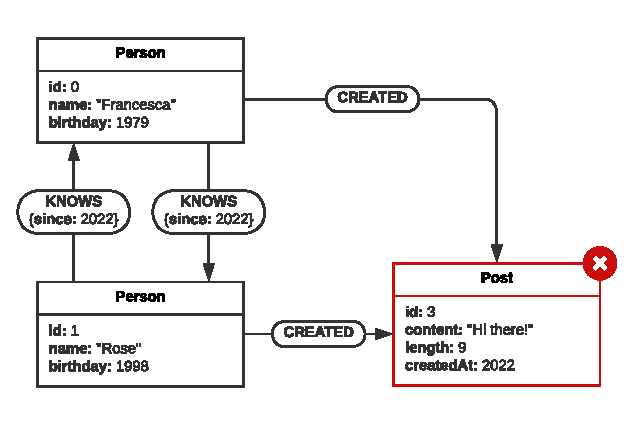
\includegraphics[width=\textwidth]{figures/conformance-too-many-in.pdf}
    \caption{This \texttt{Post} has too many incoming \texttt{created} edges, which violates rule \ref{rule:conformance-in}.}
    \label{fig:conformance-edge-target}
  \end{subfigure}
  \hfill
  \begin{subfigure}[t]{0.45\textwidth}
    \centering
    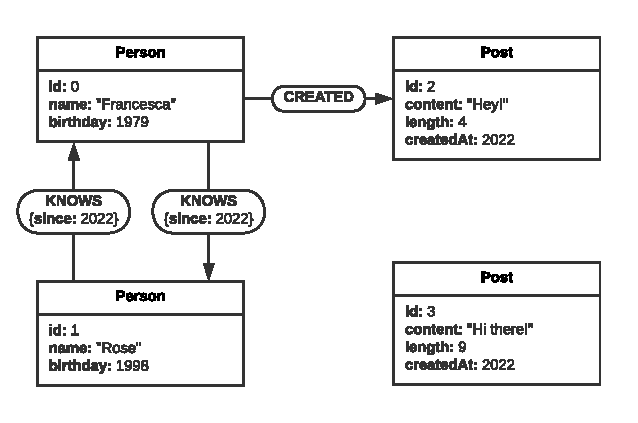
\includegraphics[width=\textwidth]{figures/conformance-basic-in.pdf}
    \caption{A \texttt{Post} is missing an incoming \texttt{created} edge, which violates rule \ref{rule:conformance-in}.}
    \label{fig:conformance-out}
  \end{subfigure}

  \caption{Examples of property graphs validated against the schema of \autoref{fig:pg-schema}. Violating nodes and edges have a red dotted outline.}
  \label{fig:conformance}
\end{figure}

\subsection{Optional properties}
\label{sec:optional-properties}

We revise the definition of record by adding a special property value $\undefined$, which indicates that the value of a property is not defined. The following definitions supersede Definition~\ref{def:record-basic}, \ref{def:property-conformance-basic}, \ref{def:record-type-basic}, and \ref{def:record-conformance-basic}.

\begin{definition}[Record]
  \label{def:record}
  A \emph{record} is a total function $r : \mathcal{N} \to \mathcal{V} \cup \{\undefined\}$ that maps property names to property values or the special value $\undefined$. The set of all records is denoted as $\mathcal{R}$.
\end{definition}

For a record $r$ and a property name $k \in \mathcal{N}$ such that $r(k)$ was previously undefined, we now say $r(k) = \undefined$. This can be seen as the ``default'' value of a property.

We adjust the definitions of property conformance, record type, and record conformance accordingly.

\begin{definition}[Property conformance]
  \label{def:property-conformance}
  For each property type $\ptype \in \ptypes$ there is a set $\sem{\ptype} \subseteq \mathcal{V} \cup \{\undefined\}$ that contains all property values that \emph{conform} to the type $\ptype$. We say $\ptype$ is \emph{optional} iff $\undefined \in \sem{\ptype}$. We use the notation $\ptype?$ to mark a property as optional, i.e. $\sem{\ptype?} = \sem{\ptype} \cup \{ \undefined \}$.
\end{definition}

\begin{definition}[Record type]
  \label{def:record-type}
  A \emph{record type} is a total function $\rtype : \mathcal{N} \to \ptypes$ that maps property names to a property type.
  % We denote such record types as $\langle a_1 : \rtype_1, \ldots, a_n : \rtype_n \rangle$.
\end{definition}

\begin{definition}[Record conformance]
  \label{def:record-conformance}
  We say that a record $r$ \emph{conforms} to a record type $\rtype$, denoted $r \in \sem{\rtype}$, if and only if for each property name $k \in \mathcal{N}$ it holds that $r(k) \in \sem{\rtype(k)}$.
\end{definition}

\subsection{Open records}

It may be desirable to allow a record to have properties with any name or any value. Such \emph{open records} can already be expressed under the current definitions. For a record type $\rtype$, we can allow properties with any name by setting $\rtype(k) = \ptype?$ for all (previously unspecified) property names $k \in \mathcal{N}$, where $\ptype$ is an arbitrary property type. Note that there may be infinitely many such $k$, so in practice we may want to have a special syntax to express this. We can allow these properties to have any value by choosing a $\ptype$ such that $\sem{\ptype} = \mathcal{V}$, or we can restrict them to a subset of $\mathcal{V}$.

\section{Limitations}

Our schema formalisms come with a number of limitations. First, it is not possible to specify constraints over a graph pattern larger than two neighboring nodes and the edge between them. For example, say we want to allow a person to drive a car, but only when they have a driver's license. \autoref{fig:drivers-license} depicts a schema that models these entities and their relations this using three nodes and two edges. Unfortunately, it is not possible to prevent a person from driving a car without having a driver's license. This illustrates the limited scope of the constraints that we can specify.

\begin{figure}[t]
  \centering
  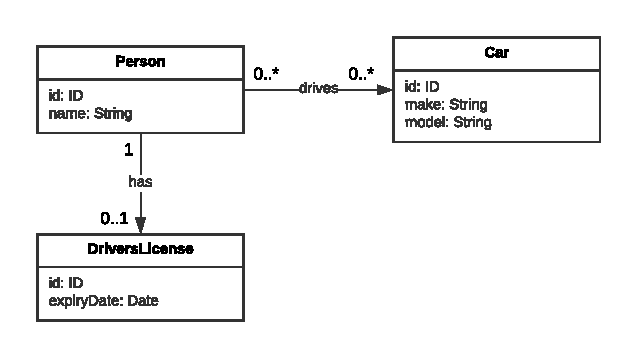
\includegraphics{figures/drivers-license.pdf}
  \caption{A schema consisting of three nodes and two edges. While we can enforce constraints on edge cardinalities, we cannot specify that a person may only drive a car if they have a driver's license.}
  \label{fig:drivers-license}
\end{figure}

% Alternatively, we can have two \texttt{Person} nodes, where one requires having a \texttt{DriversLicense} and allows owning 0 or more \texttt{Car}s, and the other does not allow owning a \texttt{Car}. This would indeed prevent a situation where a \texttt{Person} owns a \texttt{Car}, but does not have a \texttt{DriversLicense}. However, ...

% However, this breaks down when we add constraints that depend on the uniqueness of a \texttt{Person}. For example, say we want to model that a Person has exactly one Passport, and every Passport is associated with exactly one Person.
% FIXME: actually, this seems possible, as long as everything is the same for both Person nodes

% Node with any label: create a node for every combination of labels (but then we can't express there should be an edge to "at least one" of them). Solution: union types? Look into type theory again

% Furthermore, it is not possible to have a single object type that allows two different label sets. Hence, it is not possible to have optional labels, i.e. the object type $\otype = (\{\texttt{Vehicle}, \texttt{Car}\}, \langle \texttt{make} : \texttt{string} \rangle)$ requires that the labels \texttt{Vehicle} and \texttt{Car} are both present, just having \texttt{Car} is not enough. Of course, it is possible to have two schema objects like $\otype_1 = (\{\texttt{Car}\}, \langle \texttt{make} : \texttt{string} \rangle)$ and $\otype_2 = (\{\texttt{Vehicle}, \texttt{Car}\}, \langle \texttt{make} : \texttt{string} \rangle)$. However, then it is not possible to specify that every \texttt{Employee} must have exactly one outgoing \texttt{OWNS} edge to a node conforming to either $\otype_1$ or $\otype_2$.

% In general, it's not possible to say that an object must conform to type 1 OR type 2 (union type). Problem with labels follows from that. But also union of two records is not possible.

Furthermore, subtype relations cannot be expressed in general. To see the problem, consider the schema depicted in \autoref{fig:subtyping}. How could we express this using our schema formalism? An attempt is given in \autoref{fig:subtyping-ours}, where properties of the supertype \texttt{Message} are copied and distributed over all its subtypes, and the edge from \texttt{Comment} to \texttt{Message} is accompanied by an edge from \texttt{Comment} to Post and from \texttt{Comment} to itself. While the properties are modeled correctly in this case, it breaks down when we look at the cardinalities.

In \autoref{fig:subtyping}, a constraint is specified which we can express in words as ``every \texttt{Comment} is a reply of exactly one \texttt{Message} (or a subtype of \texttt{Message})''. However, it is not possible to specifiy such a constraint without subtype relations, as illustrated by \autoref{fig:subtyping-ours}. This solution allows \texttt{Comment}s which are not a reply to anything, or which are a reply to more than one thing. Then again, if we disregard the cardinality constraints, the two schemas are equivalent. This example shows that our schema formalism can be used to model some but not all subtype relations.

\begin{figure}[t]
  \centering
  \begin{subfigure}[t]{0.45\textwidth}
    \centering
    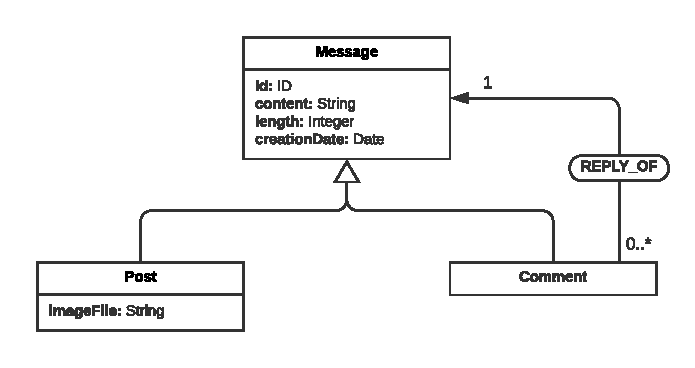
\includegraphics[width=\textwidth]{figures/subtyping.pdf}
    \caption{A schema with a subtype relation. The arrow with solid white head indicates a ``subtype of'' relation.}
    \label{fig:subtyping}
  \end{subfigure}
  \hfill
  \begin{subfigure}[t]{0.45\textwidth}
    \centering
    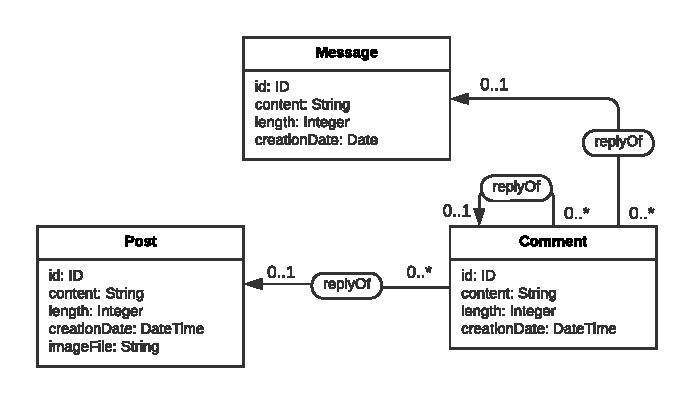
\includegraphics[width=\textwidth]{figures/subtyping-ours.pdf}
    \caption{An attempt to express the same schema without subtype relations. Note that this schema is strictly more permissive than~(a).}
    \label{fig:subtyping-ours}
  \end{subfigure}
  \caption{A schema consisting of a supertype with two subtypes which cannot be modeled using our schema formalism. Any property graph that conforms to~(a) also conforms to~(b), but not the other way around.}
\end{figure}

\bibliographystyle{apalike}
\bibliography{main}

\end{document}
